\documentclass[10pt,twocolumn,letterpaper]{article}
\usepackage[review]{cvpr}
\usepackage{microtype}
\usepackage{mathtools}
\usepackage{multirow}
\usepackage{array}
\usepackage{float}
\usepackage{siunitx}
% Evaluate the official template's length expression before passing it to
% LenToUnit. Older LaTeX picture backends otherwise print a literal "-12pt".
\makeatletter
\let\cvprOriginalLenToUnit\LenToUnit
\renewcommand{\LenToUnit}[1]{\expandafter\cvprOriginalLenToUnit\expandafter{\the\dimexpr#1\relax}}
% Restore the full usable column height after flushing wide and single floats.
\newcommand{\clearfullpage}{%
  \clearpage
  \global\@colroom\@colht
  \global\vsize\@colht
}
\makeatother
\sisetup{detect-all}
\newcommand{\R}{\mathbb{R}}
\newcommand{\T}{^{\mathsf T}}
\newcommand{\keycld}{KeyCLD}
\newcommand{\statee}{State--Euler}
\newcommand{\stater}{State--RK4}
\newcommand{\rms}{\operatorname{RMS}}
\newcommand{\diag}{\operatorname{diag}}
\newcommand{\rank}{\operatorname{rank}}
\newcommand{\dd}{\mathrm{d}}
\newcommand{\Nm}{\mathrm{N\,m}}
\newcommand{\mm}{\mathrm{mm}}
\newcommand{\keytitle}{Beyond Geometric Closure: Measuring and Diagnosing Mechanical Consistency in Visual Dynamics}
\definecolor{cvprblue}{rgb}{0.21,0.49,0.74}
\usepackage[pagebackref,breaklinks,colorlinks,allcolors=cvprblue]{hyperref}
\usepackage[capitalize,nameinlink]{cleveref}
\hypersetup{pdftitle={Beyond Geometric Closure: Measuring and Diagnosing Mechanical Consistency in Visual Dynamics},
            pdfauthor={Anonymous},pdfsubject={CVPR-format research draft}}

\def\paperID{DRAFT}
\def\confName{CVPR}
\def\confYear{}
\title{\keytitle}
\author{Anonymous Authors}
\begin{document}
\setlength{\dbltextfloatsep}{10pt plus 2pt minus 2pt}
\setlength{\textfloatsep}{10pt plus 2pt minus 2pt}
\maketitle

\begin{abstract}
Visual accuracy, geometric validity, and agreement with applied forces are distinct requirements for visual dynamics. We introduce a diagnostic framework that connects reaction-free SI measurements to controlled interventions on coordinate readout, training integration, and actuator response. Reference replay calibrates the measurement path, while continuous scoring exposes progress against fixed engineering targets. With three seeds per setting, we evaluate KeyCLD and CON across 343 planar assemblies at $64/256$ pixels and V-JEPA + AC and LingBot-VA on 100 shared spatial test assemblies. CON reduces image MSE by $37.6\%/37.2\%$ relative to persistence, yet neither planar model attains valid native geometry. At 256 pixels, calibrated RGB replay places forecast errors far above the reference measurement floor. Exact-state KeyCLD has identical geometric pass rates under Euler and RK4 training, yet its score rises from 52.65 to 64.30 as force and energy errors decrease. In both spatial pathways, CAD/IK reconstruction restores geometry while mean actuator residuals exceed five times the engineering targets. These diagnoses distinguish coordinate correction, numerical improvement, and persistent force-response errors, guiding targeted improvements to visual dynamics.
\end{abstract}

\section{Introduction}
\label{sec:intro}
Predicting motion from images and actions is central to embodied interaction. Mechanical consistency requires that motion agree with independently specified geometry, actuator inputs, and work in SI units.

Rigid closed chains make the distinction concrete: closure fixes admissible shapes, while speed and acceleration along the same path determine actuator demands. In our exact-state KeyCLD controls, Euler and RK4 training both pass every geometric check, yet mean torque residuals fall from 4.56 to 0.72 N\,m (Table~\ref{tab:corpus}). The identical geometry scores leave a mechanically important difference unresolved.

Our framework connects physical residuals to interventions that distinguish their sources. Geometry checks and reaction-free force and energy measurements establish the discrepancies (\cref{fig:audit}), with reference replay calibrating the measurement path. Readout changes, paired training integrators, and fixed-state torque perturbations then distinguish coordinate, numerical, and constitutive errors.

\begin{figure*}[t]
\centering
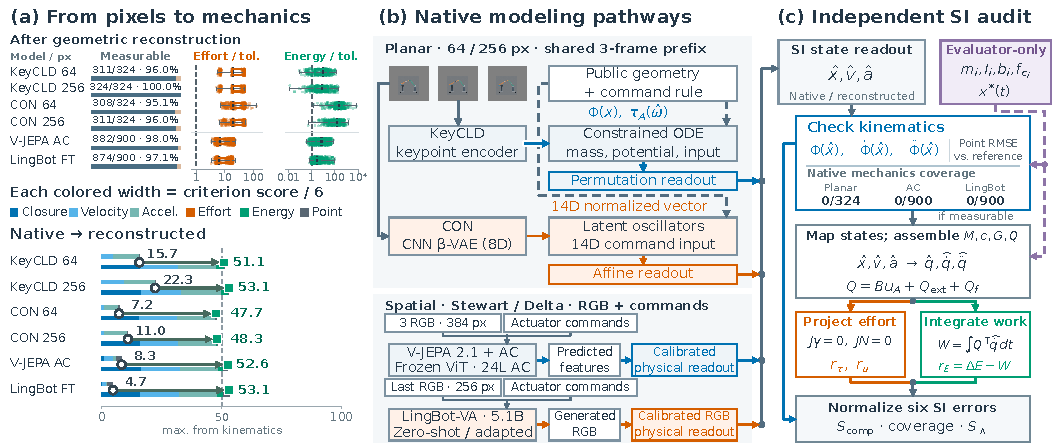
\includegraphics[width=\textwidth]{figures/audit_mechanism.pdf}
\caption{Four pathways from pixels to mechanics. (a) After reconstruction, blue/tan bars show measurable/unavailable fractions, with measurable/total counts and percentages. Effort/energy plots show cases, quartiles, ranges, and dashed tolerances. Below, six contributions sum to $S_{\rm comp}$; arrows show reconstruction gains and 50 marks the maximum kinematic contribution. Scores use task-specific targets with balanced seeds, families, and conditions; each spatial pathway contains 900 cases (LingBot FT: 50 updates). (b,c) Physical readouts feed kinematic and effort/energy tests using independent SI parameters ($B u_A=e_1\tau_A$ for planar chains).}
\label{fig:audit}
\end{figure*}

We apply the audit to constrained Lagrangian dynamics (KeyCLD)~\cite{daems2024keycld} and latent coupled oscillators (CON)~\cite{stolzle2024con} at two planar image resolutions, then to predictive features (V-JEPA 2.1 + AC)~\cite{murlabadia2026vjepa2_1,assran2025vjepa2} and generative video--action modeling (LingBot-VA)~\cite{li2026causal} on Stewart and Delta mechanisms.

We contribute (1) reaction-free evaluation separating admissibility, actuator and energy balance, and tracking through six SI criteria; (2) calibrated interventions identifying errors concealed by aggregate prediction scores; and (3) planar and spatial benchmarks establishing these distinctions across four modeling paradigms.

\section{Related Work}
\label{sec:related}
\paragraph{Mechanical foundations.}
Hamiltonian~\cite{greydanus2019hamiltonian} and Lagrangian networks~\cite{cranmer2020lagrangian,lutter2019delan}, Cartesian constraints~\cite{finzi2020constraints}, and dissipative SymODEN~\cite{zhong2020dissipative} encode energy, geometry, and velocity-dependent forces. These priors and their analyses~\cite{gruver2022deconstructing} inform our diagnostics.

\paragraph{Learning physical evolution from images.}
Physion studies physical prediction from vision~\cite{bear2021physion}. Hamiltonian Generative Networks~\cite{toth2020hgn} and coordinate-aware Lagrangian models~\cite{zhong2020images} link images to mechanics. Our four evaluated pathways span constrained keypoints, latent oscillators, predictive features, and video--action generation; Sections~\ref{sec:design} and~\ref{sec:spatial} specify their objectives and diagnostic controls.

\paragraph{Visual physics evaluation.}
Physics-IQ measures continuation fidelity~\cite{motamed2026physicsiq}, while MechVerse tests coupling between mechanical parts~\cite{jain2026mechverse}. Morpheus evaluates governing equations and physical invariants~\cite{tragoudaras2026morpheus}; WorldBench estimates calibrated parameters~\cite{upadhyay2026worldbench}, and Last Exam tests scale-free physical relationships~\cite{gao2026lastexam}. GAUGE's video-model branch separates equation form from parameter and force--motion consistency~\cite{wang2026gauge}.

\paragraph{From evaluation to diagnosis and learning.}
RigidBench intervenes on position-related representations~\cite{jain2026rigidbench}, while WorldModelBench and PISA connect evaluation to reward-based post-training~\cite{li2025worldmodelbench,li2025pisa}. We extend physical evaluation to the sources of closed-chain error. Eliminating internal reactions fixes the residual in actuator units; paired readout, integrator, and force interventions distinguish coordinate correction, numerical improvement, and response calibration within geometrically valid motion.

\section{Measuring Mechanical Consistency}
\label{sec:audit}
\subsection{Physical coordinates and admissible acceleration}
We derive the audit for a planar chain with fixed ground, one driven crank, and independent coordinate $\theta=q_1$; Section~\ref{sec:spatial} extends it to space. For 4R chains, $q=(q_1,q_2,q_3)$ are absolute link angles, $(l_1,l_2,l_3)$ are link lengths, and $d$ is anchor spacing. With $e(\psi)=(\cos\psi,\sin\psi)\T$, closure is
\begin{equation}
\phi(q)=l_1e(q_1)+l_2e(q_2)-l_3e(q_3)-(d,0)\T=0.
\label{eq:closure}
\end{equation}
For a crank-slider, $q_3$ is the slider position $s$ and the last two terms become $-(s,h_s)\T$, where $h_s$ is guide offset. Crank-rocker and double-crank geometries share the 4R topology.

The physical audit uses hinges $B,C$ and the coupler midpoint $P$ as $x=(B,C,P)\in\R^6$. With fixed anchors $A,D$, the five point constraints are
\begin{equation}
\begin{aligned}
\Phi(x)=\bigl(&\|B-A\|-l_1,\ \|C-B\|-l_2,\\
&\|C-D\|-l_3,\ [P-(B+C)/2]\T\bigr)\T.
\end{aligned}
\label{eq:pointconstraints}
\end{equation}
The set $\Phi(x)=0$ is the configuration manifold: five independent constraints leave one degree of freedom in six point coordinates. For the slider, guide height replaces the third constraint. Calibrated readouts give metre-valued $x$; rod directions give link angles through $\operatorname{atan2}(r_z,r_x)$, and $C_x$ gives slider position. We check raw $\Phi(\hat x)$ before conversion. Geometry and camera calibration are public; mass, inertia, and friction enter the independent evaluator.

Let $J=\partial\phi/\partial q$ and $\gamma=\partial q/\partial\theta$. The tangent $\gamma$ describes how all links move when the crank advances by one radian. It satisfies $J\gamma=0$ and $\gamma_1=1$. With $\gamma'=\partial\gamma/\partial\theta$, regular configurations obey
\begin{equation}
\dot q=\gamma\omega,\qquad
\ddot q=\gamma\alpha+\gamma'\omega^2,
\quad \omega=\dot\theta,\ \alpha=\ddot\theta.
\label{eq:admissible}
\end{equation}
The first term changes crank speed; the second follows the curved path even at constant speed. Closure fixes this path but leaves the tangent acceleration $\alpha$ to force balance.

\paragraph{Constraint preservation needs a correct initial level.}
KeyCLD's acceleration-level enforcement gives
\begin{equation}
D\Phi\,\ddot x+D^2\Phi[\dot x,\dot x]=0
\ \Longrightarrow\
\Phi(x(t))=\Phi(x_0)+tD\Phi(x_0)\dot x_0.
\label{eq:levelset}
\end{equation}
Velocity projection removes the second term, leaving the initial closure residual unchanged. Consequently, acceleration-level enforcement preserves the geometry supplied by the visual initialization, including incorrectly decoded rod lengths. This distinction motivates separate tests of coordinate anchoring and subsequent dynamics.

\subsection{Independent rigid-body forces}
Reference rigid-body properties determine the independent mass matrix $M$, velocity bias $c$, and gravity $G$. Application-point Jacobians map external forces, while $Q_f$ combines viscous and smooth Coulomb friction in relative joint velocities (supplementary derivation).

With $e_1=(1,0,0)\T$ selecting the driven crank and $\lambda$ denoting constraint reactions, the full equation is
\begin{equation}
M\ddot q+c+G=e_1\tau_A+Q_{\rm ext}+Q_f+J\T\lambda.
\label{eq:dynamics}
\end{equation}
Joint reactions keep the chain joined but do no work along its permitted motion. Because $J\gamma=0$, projection onto $\gamma$ removes these unknown forces and exposes the predicted crank-torque mismatch:
\begin{equation}
r_\tau=\gamma\T\!\left[M\widehat{\ddot q}+c+G-Q_{\rm ext}-Q_f\right]-\tau_A.
\label{eq:torque}
\end{equation}
Every term is evaluated at the predicted state. The normalization $\gamma_1=1$ gives $r_\tau$ the scale of the actual crank torque. The effective inertia $\mathcal I=\gamma\T M\gamma$ measures all moving bodies' resistance to crank acceleration; the supplement derives the corresponding reduced dynamics.

\subsection{Six complementary physical criteria}
The independent energy is $E=\tfrac12\dot q\T M\dot q+\sum_i m_i g e_z\T p_i$, where $p_i$ is body $i$'s center of mass and $e_z$ points upward. The generalized force $Q=e_1\tau_A+Q_{\rm ext}+Q_f$ collects motor, external, and friction forces; $Q\T\dot q$ is their total power. The work--energy residual compares energy change with supplied work:
\begin{equation}
r_E(t)=E(t)-E(t_0)-\int_{t_0}^t Q\T\dot q\,\dd t.
\label{eq:energy}
\end{equation}
For admissible motion, $r_E(t)=\int_{t_0}^t r_\tau(s)\omega(s)\,\dd s$. The torque residual tests local force balance, whereas the energy residual accumulates its effect along the motion. Because power vanishes at rest even when forces are incorrect, the two measurements provide complementary evidence.

The six criteria separate admissibility, mechanics, and tracking. Closure uses maximum absolute $\Phi(\hat x)$; tangent velocity and curvature-consistent acceleration use maximum-channel RMS of $\dot\Phi=D\Phi\hat v$ and $\ddot\Phi=D\Phi\hat a+D^2\Phi[\hat v,\hat v]$. Force and energy errors are RMS $r_\tau$ and maximum absolute prefix $r_E$. Finally, maximum-channel RMS of $\hat x-x^*$ tests whether the motion follows the reference trajectory, since an admissible path can still have the wrong phase. All use future samples, with $\hat v,\hat a$ supplied by the native ODE.

\begin{table}[t]
\caption{Engineering targets fixed by task and shared by its models. Torque/servo columns are planar; spatial effort and work scales follow Section~\ref{sec:spatial}.}
\label{tab:criteria}
\centering\small
\setlength{\tabcolsep}{3pt}
\begin{tabular}{lrrr}
\toprule
Criterion & Torque & Servo & Spatial\\
\midrule
Closure & $1$ mm & $1$ mm & $1$ mm\\
Velocity & $.01$ m/s & $.01$ m/s & $.01$ m/s\\
Acceleration & $.1$ m/s$^2$ & $.1$ m/s$^2$ & $.1$ m/s$^2$\\
Actuator RMS & $.1$ N\,m & $.25$ N\,m & $5\%$ rated\\
Energy defect & $.02$ J & $.05$ J & $1\%$ work\\
Point RMSE & $1$ cm & $1$ cm & $1$ cm\\
\bottomrule
\end{tabular}
\end{table}

\begin{figure*}[t]
\centering
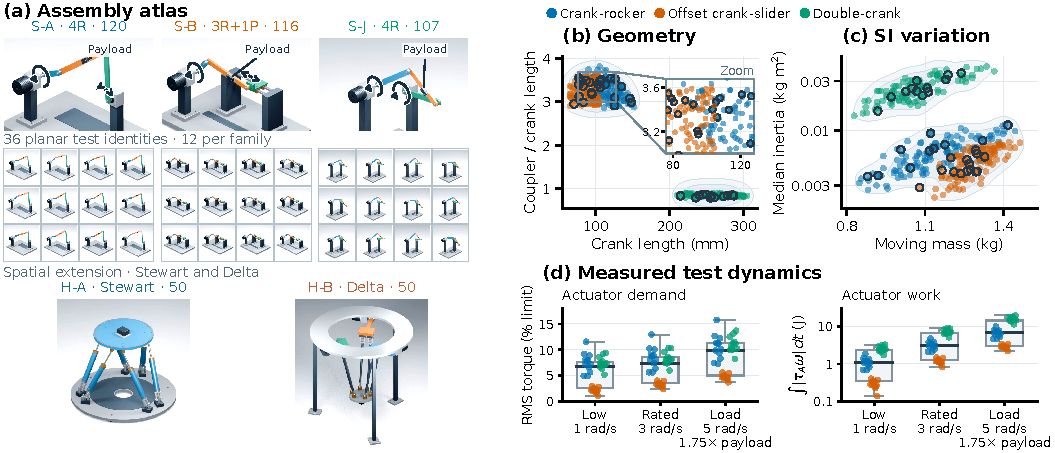
\includegraphics[width=\textwidth]{figures/corpus_overview.pdf}
\caption{Assembly corpus. (a) Three planar families and their 36 test identities, with Stewart/Delta examples. (b--d) Planar distributions: density contours cover 343 assemblies, test identities are ringed, and inertia is median over 41 poses. Torque and absolute work use 36 references per condition; boxes/whiskers show quartiles/ranges, and torque is normalized by actuator limits.}
\label{fig:mechanisms}
\end{figure*}

\paragraph{Continuous scoring at fixed engineering targets.}
The tolerances in Table~\ref{tab:criteria} express task requirements and are fixed before model evaluation. For case $i$ and criterion $k$, let $m_{ik}=1$ when its complete residual is measurable and $\rho_{ik}=r_{ik}/\tau_{ik}$ be its error-to-tolerance ratio. We use one continuous composite, with strict joint qualification as an auxiliary:
\begin{equation}
\begin{aligned}
S_{\rm comp}&=\frac{100}{6}\sum_{k=1}^6\left\langle\frac{m_{ik}}{1+\rho_{ik}^2}\right\rangle_{\rm bal},\\
S_{\land}&=100\left\langle\prod_{k=1}^6 m_{ik}\,\mathbf{1}[\rho_{ik}\le1]\right\rangle_{\rm bal}.
\end{aligned}
\label{eq:scores}
\end{equation}
Each criterion scores 100 at zero error, 50 at tolerance, and 20 at twice tolerance. Three exact kinematic criteria already contribute 50 composite points, so $S_{\rm comp}\ge50$ does not imply joint qualification. All registered cases retain the six-term denominator, with missing terms contributing zero. We average registered trajectories within conditions, then conditions, families, and seeds equally. Physical coverage counts cases with all six measurements, whereas $S_{\land}$ additionally requires all six to pass.

\paragraph{Calibrating the measurement path.}
Closure measures agreement with supplied rod lengths, whereas localization measures agreement with reference coordinates. A hard constraint can preserve the former even at $64\times64$, so resolution changes the reader's calibration rather than the engineering target. To measure the instrument's contribution, we process reference and predicted RGB or features through the same frozen reader, reconstruction, and differentiator. Exact-state replay first isolates numerical error: quintic splines pass all six criteria on 54/54 planar reference trajectories. Correct-video replay then adds visual localization error, providing the reference against which forecast residuals are interpreted.

\section{Experimental Design}
\label{sec:design}
The 30 Hz planar study separates resolution, anchoring, and integration (Section~\ref{sec:results}). Torque excitation at 100 Hz then isolates constitutive response (Section~\ref{sec:structure}), followed by predictive features and generated video under spatial position control (Section~\ref{sec:spatial}).

\subsection{Shared assembly corpus}
MuJoCo~\cite{todorov2012mujoco} trajectories rendered in Blender span 343 crank-rockers, offset sliders, and double-cranks with varied geometry and rigid-body properties (\cref{fig:mechanisms}). We partition them into 271 training, 18 validation, 18 calibration, and 36 test identities, keeping each assembly's conditions and views together. Three conditions yield 108 test sequences per seed.

Both video models train independently at $64\times64$ and $256\times256$, sampled directly from the same source renders with a $1.30$ m field of view. Splits, motions, commands, and SI targets are shared. Each model observes three frames from $1$ s, trains on 50-frame windows, and forecasts through $3.967$ s. Commands are $1$, $3$, and $5$ rad/s, with $1.75\times$ payload at the highest speed. The public controller converts predicted crank velocity to torque:
\begin{equation}
\tau_A=\operatorname{clip}[k_p(\omega_{\rm cmd}-\widehat\omega),-\tau_{\max},\tau_{\max}].
\label{eq:servo}
\end{equation}
Crank-rockers and sliders use $k_p=2$ N\,m\,s/rad and $\tau_{\max}=5\,\Nm$; double-cranks use $k_p=12$ N\,m\,s/rad and $\tau_{\max}=12\,\Nm$. The common $0.25\,\Nm$ criterion specifies absolute precision across these actuator scales. Forecasts use observed prefixes and public commands; future measured torque and reference states enter only the evaluator.

\subsection{Native objectives and diagnostic controls}
Each model retains its released architecture and native objective, with geometry and command interfaces adapted to the shared corpus. Interventions define the diagnostic comparisons: a changed readout holds forecasts fixed, exact-state controls remove visual initialization error, and paired training integrators hold initialization, data order, objective, and budget fixed.

KeyCLD combines image/heatmap reconstruction with four-step constrained prediction. CON jointly trains its CNN $\beta$-VAE and eight-coordinate oscillators over 50-frame windows~\cite{stolzle2024con}. Figure~\ref{fig:audit}b defines their respective torque/command interfaces.

\begin{figure*}[t]
\centering
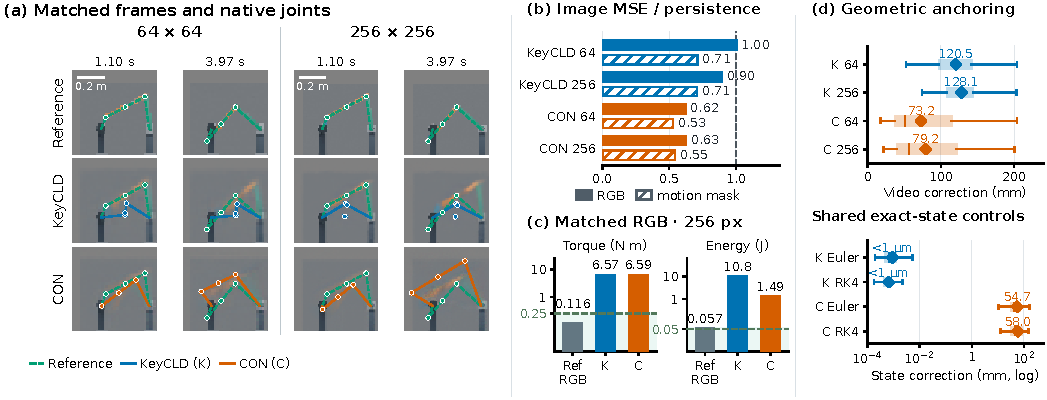
\includegraphics[width=\textwidth]{figures/shared_video_audit.pdf}
\caption{Matched resolution and measurement controls. (a) The first test case, seed 42, at both resolutions; dashed/solid skeletons show reference/native joints. (b) Labeled mean MSE ratios to same-resolution persistence; solid/hatched bars show RGB/motion mask, and lower is better. (c) Correct and generated RGB through one frozen reader and phase differentiator; dashed lines mark SI targets. (d) Reconstruction costs: diamonds show balanced means, boxes quartiles, whiskers full ranges.}
\label{fig:shared-video}
\end{figure*}

\begin{table*}[t]
\caption{Planar audit, 324 tests per row. Finite / Phys. / Cov. count finite outputs / native SI coverage / reconstructed SI coverage. Percentages are pass rates; G/V/A denote closure/velocity/acceleration. N/A marks unavailable mechanics. $S_{\rm comp}$ gives three-seed mean$\pm$SD. Reconstructed errors are available-case means balanced by seed/family/condition; correction is coordinate RMS and point error maximum-channel RMSE. State controls are resolution-independent. Persistence RGB MSE is 4.94/5.04 at 64/256 pixels in the displayed units.}
\label{tab:corpus}
\label{tab:geometry-readout}
\centering\small
\setlength{\tabcolsep}{1.7pt}
\begin{tabular}{@{}lrrrrrrrrr@{\hspace{5pt}}rrrrr@{}}
\toprule
& \multicolumn{9}{c}{Native output} & \multicolumn{5}{c}{After geometric reconstruction}\\
\cmidrule(lr){2-10}\cmidrule(l){11-15}
Training & Finite & \shortstack{RGB MSE\\($10^{-4}$)} & Phys. & \shortstack{G / V / A\\(\%)} & \shortstack{Torque\\(\%)} & \shortstack{Energy\\(\%)} & \shortstack{Point\\(mm)} & \shortstack{Joint\\(\%)} & \shortstack{$S_{\rm comp}$\\(0--100)$\uparrow$} & Cov. & \shortstack{Correction\\(mm)} & \shortstack{Torque\\(N\,m)} & \shortstack{Energy\\(J)} & \shortstack{Point\\(mm)}\\
\midrule
\multicolumn{15}{l}{\textit{KeyCLD}}\\
Video 64 px & 311 & 4.96 & 0 & 0/22.2/65.1 & N/A & N/A & 229.2 & 0 & $15.73\pm5.00$ & 311 & 120.49 & 6.383 & 0.921 & 194.80 \\
Video 256 px & 324 & 4.52 & 0 & 0/53.7/75 & N/A & N/A & 233.9 & 0 & $22.30\pm12.08$ & 324 & 128.13 & 6.229 & 1.201 & 198.19 \\
State--Euler & 324 & -- & 324 & 100/100/100 & 8.33 & 0.00 & 139.1 & 0 & $52.65\pm0.02$ & 324 & $<0.001$ & 4.564 & 22.453 & 139.06 \\
State--RK4 & 324 & -- & 324 & 100/100/100 & 7.41 & 0.00 & 16.4 & 0 & $64.30\pm0.07$ & 324 & $<0.001$ & 0.715 & 2.925 & 16.37 \\
\midrule
\multicolumn{15}{l}{\textit{CON}}\\
Video 64 px & 324 & 3.08 & 0 & 0/0.9/33 & N/A & N/A & 123.5 & 0 & $7.23\pm3.23$ & 308 & 73.18 & 6.859 & 17.960 & 154.83 \\
Video 256 px & 324 & 3.17 & 0 & 0/0/63.6 & N/A & N/A & 134.6 & 0 & $10.96\pm2.50$ & 311 & 79.17 & 6.691 & 10.470 & 167.35 \\
State--Dopri5 & 324 & -- & 0 & 0/0/3.4 & N/A & N/A & 142.4 & 0 & $1.91\pm0.79$ & 323 & 67.68 & 6.549 & 23.282 & 132.28 \\
State--Euler & 324 & -- & 0 & 0/0/4.3 & N/A & N/A & 124.5 & 0 & $2.36\pm0.46$ & 317 & 54.73 & 6.028 & 11.847 & 133.06 \\
State--RK4 & 324 & -- & 0 & 0/0/3.4 & N/A & N/A & 137.4 & 0 & $1.97\pm0.84$ & 322 & 58.01 & 6.541 & 20.476 & 132.86 \\

\bottomrule
\end{tabular}
\end{table*}

At each resolution, KeyCLD/CON complete 40/50 epochs and 32,520/40,650 sequence exposures, using batches of 1/16 and hence 32,520/2,550 updates. The supplement details native image-layer scaling and pixel-loss normalization.

A validation-selected permutation maps KeyCLD keypoints to joints, while CON uses a training-label affine map. We freeze these readouts for evaluation and isolate dynamics with exact-state controls that supply true training states and prefix velocities.

Seeds 42--44 give twelve video fits and fifteen resolution-independent state fits, evaluated at fixed final epochs. Confidence intervals use 2,000 seed/assembly resamples with conditions paired. Native-derivative calibration passes 54/54 references and rejects static and time-scaled controls.

\begin{figure*}[t]
\centering
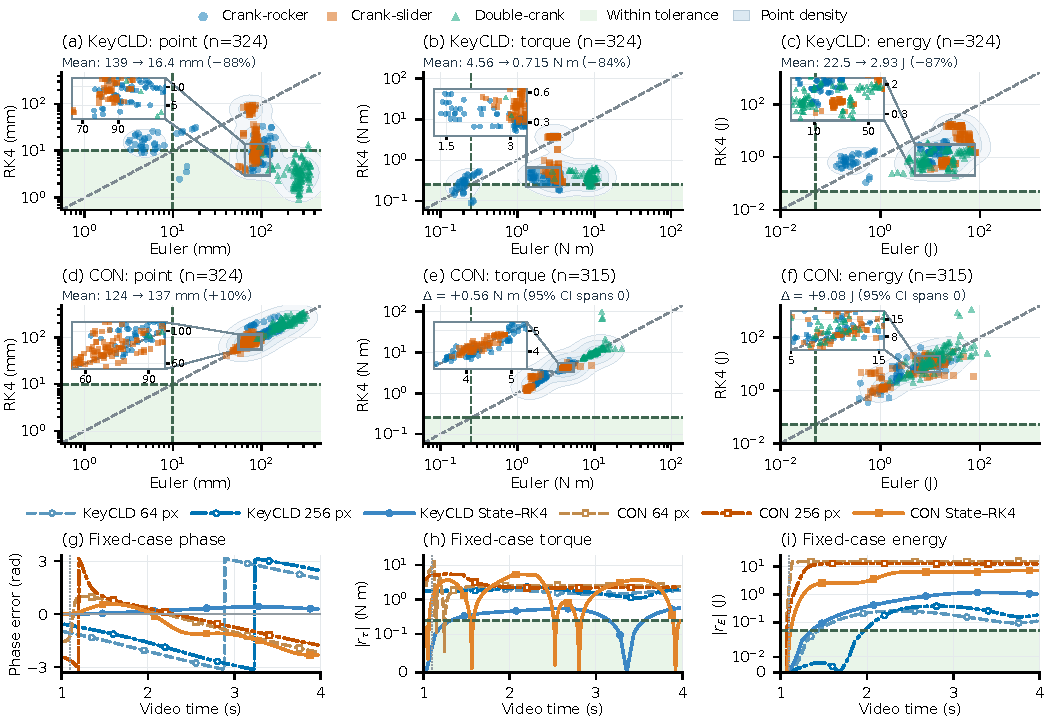
\includegraphics[width=\textwidth]{figures/corpus_paired_residuals.pdf}
\caption{Integration and resolution controls. (a--f) Resolution-independent Euler/RK4 pairs compare native point error and reconstructed force/energy; below-diagonal points favor RK4. (g--i) Six curves share one case, seed 42, time window, and geometric readout. Green bands mark tolerances; vertical dotted lines start forecasting.}
\label{fig:corpus-residuals}
\end{figure*}

\section{Shared Assembly Results}
\label{sec:results}
\subsection{Resolution intervention}
Retaining CON's native fully connected image layers expands its parameter count from 67.3M to 1.08B at $64\!\to\!256$ pixels, with 2,550 updates at either resolution. Its RGB gains over persistence remain $37.6\%/37.2\%$, with motion-region gains at both resolutions (Fig.~\ref{fig:shared-video}a,b). KeyCLD moves from near persistence to a $10.4\%$ mean RGB gain, and all 256-pixel forecasts are finite. These visual gains coexist with failed native geometry in all four settings (Table~\ref{tab:corpus}), separating visual prediction from physical coordinate anchoring under the fixed training budgets.

Continuous scores reveal which errors change. KeyCLD rises from 15.73 to 22.30 and CON from 7.23 to 10.96, mainly through velocity/acceleration consistency. Point scores remain below 1/100 at 256 pixels, and KeyCLD's seed SD reaches 12.08. Thus the higher aggregate score describes differential consistency rather than accurate tracking.

\paragraph{A common RGB measurement path.}
On identical future frames, resolution-specific readers reduce correct-video Euclidean error from 2.13 to 0.334 mm, while 256-pixel forecast errors remain 195.0/208.5 mm for KeyCLD/CON. Passing correct and generated RGB through the same frozen phase path gives torque residuals of 0.116 versus 6.57/6.59 N\,m (Fig.~\ref{fig:shared-video}c). Reference energy error is 0.057 J, close to the 0.05 J target. The calibrated gap persists at 256 pixels, motivating state and force probes of its dynamical sources.

\subsection{What changes when the state is known?}
Exact training states and prefix velocities remove visual initialization error. KeyCLD's Euler and RK4 controls both pass all three kinematic criteria on 324/324 tests, while both have zero joint qualification (Table~\ref{tab:corpus}). These matching pass rates conceal a large numerical improvement: RK4 training reduces torque and energy residuals by more than $84\%$ and raises $S_{\rm comp}$ from 52.65 to 64.30 (Fig.~\ref{fig:corpus-residuals}). The paired control locates an integration-dependent error within geometrically valid motion; the remaining energy failures identify the unresolved work imbalance.

CON evolves six Cartesian coordinates padded to eight oscillator coordinates, so it must learn their curved one-dimensional admissible manifold. Its forecasts violate geometry, and RK4 increases native point error by $12.907$ mm (95\% interval $[6.734,23.497]$). Higher-order integration therefore has opposite effects on trajectory accuracy in the two pipelines.

\begin{figure*}[t]
\centering
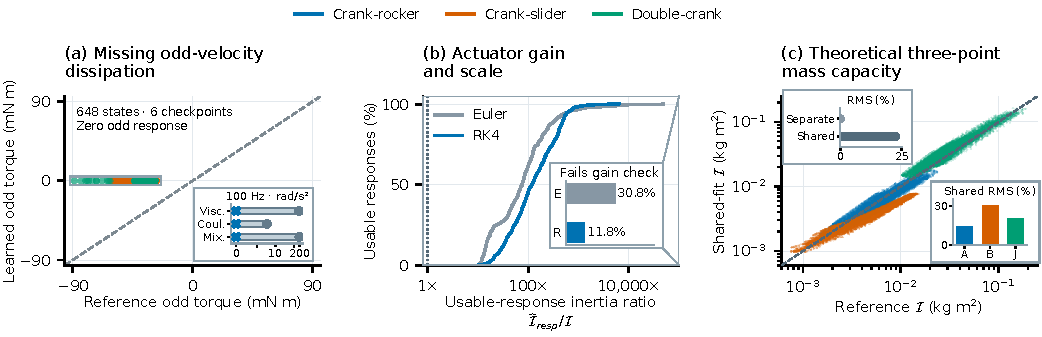
\includegraphics[width=\textwidth]{figures/constitutive_evidence.pdf}
\caption{Structural evidence. (a) Six checkpoints give zero odd torque on 648 states. The 100 Hz inset compares RMS odd acceleration (reference bars/dots, model crosses; symlog scale). (b) Each integrator pools 1,944 queries; the inset shows failed gain checks. (c) Mass fits use 44,280 poses, with separate/shared and family errors in the insets.}
\label{fig:constitutive}
\end{figure*}

\subsection{Force and energy after a common geometric readout}
For each saved forecast, predicted crank direction and derivatives define a causal reconstruction using public geometry. Its coordinate correction quantifies the cost of recovering admissible motion. Large video corrections persist at both resolutions (Fig.~\ref{fig:shared-video}d), whereas exact-state KeyCLD needs less than a micrometer and CON's state arms need $54.7$--$67.7$ mm. Reconstruction raises 256-pixel $S_{\rm comp}$ to 53.10/48.26 for KeyCLD/CON by restoring geometric terms, while torque, energy, and point errors remain above target (Table~\ref{tab:geometry-readout}). Matched traces (Fig.~\ref{fig:corpus-residuals}g--i) show phase drift and above-target mechanical defects at both resolutions.

\section{Structural and Intervention Analysis}
\label{sec:structure}
KeyCLD's torque interface lets us test whether improved rollouts also yield calibrated force response. Velocity reversal, torque perturbation, and mass-capacity fits distinguish dissipation, actuator scale, and cross-assembly parameter sharing (Fig.~\ref{fig:constitutive}).

\subsection{Torque excitation: dissipation and calibration}
The torque-excitation protocol removes servo feedback so that commanded torque directly specifies the intervention. KeyCLD trains on a frictionless four-bar at 100 Hz under $[-2,2]\,\Nm$ torques; eight friction, load, scale, and topology conditions then provide 96 calibration and 160 transfer trajectories.

At fixed pose and torque, KeyCLD's force $f(x,u)=-\nabla V(x)+B(x)u$ is velocity-independent and its constraint-curvature term is quadratic in velocity. Its acceleration is therefore unchanged by reversal. The half-difference isolates friction's odd response, cancelling gravity and other velocity-even terms:
\begin{equation}
\frac{\alpha(\theta,\omega,\tau)-\alpha(\theta,-\omega,\tau)}{2}
=-\frac{\mathcal F(\theta,\omega)}{\mathcal I(\theta)}.
\label{eq:odd}
\end{equation}
All 292 reversal pairs per friction condition have zero learned odd acceleration. The nonzero viscous, Coulomb, and mixed-friction references in Fig.~\ref{fig:constitutive}(a) expose a representational restriction, consistent with the missing dissipation identified by KeyCLD~\cite{daems2024keycld}.

Rescaling $(M_x,V,B)\mapsto(kM_x,kV,kB)$, $k>0$, preserves acceleration, so motion fitting alone cannot identify absolute SI parameter scales. We test acceleration under a calibrated torque perturbation at fixed pose and zero speed:
\begin{equation}
k_\tau=\frac{\hat\alpha(+\delta\tau)-\hat\alpha(-\delta\tau)}{2\delta\tau},
\qquad \widehat{\mathcal I}_{\rm resp}=1/k_\tau.
\label{eq:gain}
\end{equation}
For the physical mechanism, $k_\tau=1/\mathcal I$: a larger inertia produces less acceleration per unit torque. Comparing reference and learned gains therefore tests the combined calibration of inertia and actuation.

\begin{figure*}[t]
\centering
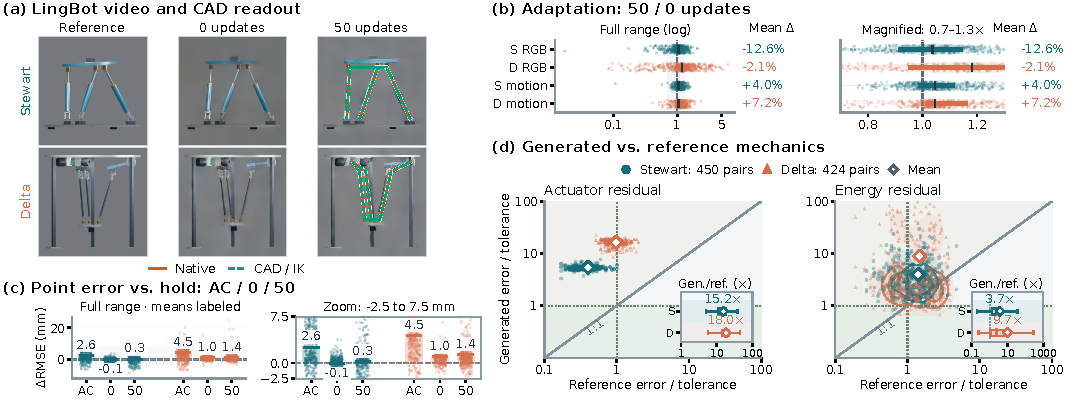
\includegraphics[width=\textwidth]{figures/spatial_vjepa_audit.pdf}
\caption{Spatial diagnostics. (a) LingBot video and CAD readouts. (b) Paired 50/0-update MSE ratios. (c) Finite point errors and mean bars (450 registered per setting/family). (d) Mechanics on 450 Stewart and 424 Delta pairs. Warm/green regions mark errors above reference/within tolerance; contours show density, diamonds means, and insets paired-ratio quartiles, ranges, and means.}
\label{fig:spatial}
\end{figure*}

\subsection{Shared assemblies: response and representation}
Each of the six frozen 30 Hz KeyCLD state checkpoints is queried at the same 648 held-out states. Holding torque fixed removes servo feedback that can resemble damping; the learned odd response remains zero. With $\delta\tau=0.25\,\Nm$ and three pooled seeds, failures of the finite, $k_\tau>10^{-8}$ gain check fall from $30.8\%$ (Euler) to $11.8\%$ (RK4). Usable responses still have median inertia ratios of $74.9\times$ and $117.3\times$ the reference. The fixed-state probe thus reveals incorrect response scaling despite RK4's lower rollout residuals.

Three-point kinetic capacity distinguishes representation size from parameter sharing. Its reduced inertia is
\begin{equation}
\mathcal I_{\rm pts}(\theta)=\sum_{i\in\{B,C,P\}}m_i
\left\|\frac{\partial p_i}{\partial\theta}\right\|^2.
\label{eq:capacity}
\end{equation}
Reference-only positive-mass fits across 360 assemblies reach numerical precision separately by condition, but one shared mass vector incurs $22.55\%$ relative RMS error (Fig.~\ref{fig:constitutive}c). Three point masses can represent individual mechanisms; sharing them across mechanisms and loads requires conditioning.

\section{Predictive and Generative Spatial Dynamics}
\label{sec:spatial}
On Stewart and Delta, both models forecast 117 future frames at 30 Hz on the same 50+50 test assemblies, three conditions, and seeds 42--44. V-JEPA trains its 24-layer AC predictor on frozen 384-pixel encoder features for 3,000 exposures per family and seed; its internal state head supplies autoregressive feedback. LingBot generates $256\times256$ RGB at 0/50 full-parameter updates (400 exposures per seed), giving 1,800 videos. Fixed measurement heads decode unconstrained (native) coordinates, with matched reference replay establishing each pathway's measurement baseline.

For either pathway, a tangent basis $N$ represents the mechanism's permitted motions. With actuator map $B$, the reaction-free residual becomes
\begin{equation}
r_u=(N\T B)^{-1}N\T[M\hat a+c+G-Q_{\rm ext}-Q_f]-u_A.
\label{eq:spatial-effort}
\end{equation}
Here $JN=0$ eliminates internal reactions, and nonsingular $N\T B$ converts the remaining imbalance to actuator units. Controllers are reevaluated at predicted states; effort targets are 7.5 N/0.75 N\,m for Stewart/Delta, while energy uses 1\% of rated effort times summed command ranges.

Unconstrained AC readouts have zero mechanical coverage. Applying the calibrated measurement head and CAD reconstruction to the same saved AC feature rollouts yields Stewart/Delta effort residuals of 41.97 N/12.42 N\,m, above matched reference values of 3.11 N/2.08 N\,m (Table~\ref{tab:spatial}).

\begingroup
\setlength{\intextsep}{5pt}
\begin{table}[H]
\caption{Spatial audit of LingBot and AC, with $150\times3$ cases per row. Step counts optimizer updates. Native/CAD give $S_{\rm comp}$ (mean $\pm$ seed SD); Mech. is CAD coverage. RGB/motion MSE units: $10^{-4}/10^{-2}$.}
\label{tab:spatial}
\centering\footnotesize
\setlength{\tabcolsep}{2.0pt}
\begin{tabular}{@{}lrrrrrr@{}}
\toprule
Family & Step & RGB & Motion & Native & CAD & Mech.\\
\midrule
Stewart & 0 & 41.67 & 2.59 & $5.67\!\pm\!0.05$ & $54.60\!\pm\!0.19$ & 450/450 \\
Stewart & 50 & 36.42 & 2.69 & $6.01\!\pm\!0.15$ & $54.31\!\pm\!0.51$ & 450/450 \\
Delta & 0 & 29.43 & 1.58 & $2.80\!\pm\!0.08$ & $43.37\!\pm\!1.17$ & 359/450 \\
Delta & 50 & 28.83 & 1.70 & $3.39\!\pm\!0.02$ & $51.92\!\pm\!1.17$ & 424/450 \\

\midrule
AC Stewart & 386 & -- & -- & $6.20\!\pm\!0.69$ & $55.11\!\pm\!1.71$ & 450/450 \\
AC Delta & 400 & -- & -- & $10.40\!\pm\!5.34$ & $50.05\!\pm\!2.71$ & 432/450 \\

\bottomrule
\end{tabular}
\end{table}
\endgroup

LingBot adaptation lowers whole-image MSE by 12.6\%/2.1\% on Stewart/Delta, while motion-region MSE rises by 4.0\%/7.2\% (Fig.~\ref{fig:spatial}b). The global visual gain thus leaves the moving foreground less accurate. Both checkpoints exceed image-persistence error and have zero native mechanics coverage.

At 50 updates, CAD/IK reconstruction restores admissible configurations with 2.11/9.06 mm correction, yet point errors remain 29.92/23.24 mm. Delta's score rises from 43.37 to 51.92 through coverage and kinematic gains, while Stewart stays near 54 (Table~\ref{tab:spatial}); neither attains strict joint qualification.

At 50 updates, matched reference/generated effort residuals are 3.01/40.51 N for Stewart and 0.733/12.32 N\,m for Delta (Fig.~\ref{fig:spatial}d). Generated effort exceeds reference on all 450/424 pairs; Delta's 30 Hz exact-coordinate differentiation contributes 0.0145 N\,m. Energy defects rise from 0.605 to 1.640 J and from 0.203 to 1.206 J, respectively. Delta's 0.203 J reference residual includes RGB readout and numerical processing. Generated defects are larger in 330/424 matched pairs, indicating energy imbalance beyond reference error.

\section{Implications and Conclusion}
\label{sec:discussion}
SI measurements and controlled interventions distinguish coordinate, numerical, and constitutive errors even when geometry checks or rollout residuals improve. External geometry supplies 50.00 of KeyCLD 256's 53.10 reconstructed points and 48.15 of adapted LingBot's 53.12 (Fig.~\ref{fig:audit}), leaving force, energy, and tracking deficits against their respective targets. These diagnoses identify concrete design requirements: coordinate anchors, velocity-dependent dissipation, calibrated SI actuator response, and parameters conditioned on geometry and load.
\par
\label{maintextend}
\clearfullpage
{\small
\bibliographystyle{ieeenat_fullname}
\bibliography{references}
}
\end{document}
